\documentclass[a4paper,12pt]{article}
\usepackage{amsmath}
\usepackage{amssymb}
\usepackage[utf8]{inputenc}
\usepackage[T1]{fontenc}
\usepackage{lmodern}
\usepackage{indentfirst}
\usepackage{geometry}
\usepackage{array}
\usepackage[pdftex]{color,graphicx}
\usepackage{subfigure}
\usepackage{afterpage}
\usepackage{setspace}
\usepackage{color}
\usepackage{wrapfig}
\usepackage{listings} 
\usepackage{datetime}
\usepackage{epstopdf}
\usepackage{hyperref}

\renewcommand{\onehalfspacing}{\setstretch{1.6}}

\geometry{tmargin=2.5cm,bmargin=2.5cm,lmargin=2.5cm,rmargin=2.5cm}
\setlength{\parindent}{1cm}
\setlength{\parskip}{0mm}

\newenvironment{lista}{
\begin{itemize}
  \setlength{\itemsep}{1pt}
  \setlength{\parskip}{0pt}
  \setlength{\parsep}{0pt}
}{\end{itemize}}

\newcommand{\linia}{\rule{\linewidth}{0.4mm}}

\definecolor{lbcolor}{rgb}{0.95,0.95,0.95}
\lstset{
  backgroundcolor=\color{lbcolor},
  tabsize=4,
  language=C++,
  captionpos=b,
  tabsize=3,
  frame=lines,
  numbers=left,
  numberstyle=\tiny,
  numbersep=5pt,
  breaklines=true,
  showstringspaces=false,
  basicstyle=\footnotesize,
  identifierstyle=\color{magenta},
  keywordstyle=\color[rgb]{0,0,1},
  commentstyle=\color{green},
  stringstyle=\color{red}
  }

\begin{document}

\noindent
\begin{tabular}{|c|p{11cm}|c|} \hline 
Michał Szczygieł & Aleksander Śmierciak & \ddmmyyyydate\today \tabularnewline
\hline 
\end{tabular}


\section*{Zadanie 6 - Rozmycie Gaussa GPU}

Celem zadania numer 6 było wdrożenie złożonego programu umożliwiającego zastosowanie filtru - rozmycie Gaussa na materiał video. Głównym założeniem tej aplikacji było zaimplementowanie własnego rozwiązania rozmycia z wykorzystaniem mocy obliczeniowej kart graficznych firmy Nvidia, za pomocą architektury CUDA. Do wykonania należało także wykorzystać dostępną bibliotekę OpenCV, która umożliwa manipulację strumieniem wejściowym video, w postaci macierzy zawierających informację o pikselach (obiektu typu \emph{Mat} ). 
\\

Poniżej została przedstawiona lista kroków do realizacji zadania:
\begin{lista}
\item pobranie argumentów
\item obliczenie gridu, bloku i pobranie liczby wątków
\item otworzyć materiał filmowy, klatka po klatce
\item zastosować filtr Gaussa poprzez dokonanie modyfikacji informacji o pikselach w każdej z klatek - obliczenia zrównoleglić z pomocą CUDA
\item zapisać kolejno zmodyfikowane klatki
\item zapisać całość po zastosowaniu odpowiedniego filtra video
\end{lista}

Do implementacja rozmycia Guassa została użyta tradycyjna metoda bazująca na przekształceniu piskeli przez macierz charakterystyczną dla rozmycia gaussa. \\

W przypadku zastosowania archtektury CUDA do obliczeń równoległych, było odpowiednie przygotowanie gridu i rozdzielenie zadania na wątki. \\

Część programu odpowiedzialna za podział:

\begin{lstlisting}
/**
 * This method based on run parameters. Calculates the amount of threads/blocks for the application use.
 *
 * @param threadCount The amount of threads.
 */
void prepareGrid(unsigned int threadCount)
{
	// Round the number of threads
	if ((threadCount % 2) == 1)
	{
		++threadCount;
	}

	// Divide into blocks
	for (int i = 512; i > 0; i--)
	{
		double blocks = (double) threadCount / i;

		if (blocks == (int) (blocks))
		{
			double divThreads = sqrt(i);
			if (divThreads == int(divThreads))
			{
				threadsOnX = int(divThreads);
				threadsOnY = int(divThreads);
			}
			else
			{
				threadsOnX = i;
				threadsOnY = 1;
			}

			break;
		}
	}
}
\end{lstlisting}

Znając specyfikację karty graficznej, na której przeprowadzone były testy programu, należało paramter wejściowy, oznaczający liczbę wątków na której działa aplikacja odpowiednio zinterpretować. Powyższy kod, dzieli na bloki (obliczanie wymiarów tzw. \emph{grid'a}) w zależności od liczby wątków. \\

Implementacja Kernela CUDA:

\begin{lstlisting}
/**
 * CUDA implementation for Gaussian blur.
 *
 * @param imageIn 		The pixel to perform.
 * @param imageOut 		The result of pixel conversion.
 * @param width			The width of frame.
 * @param height 		The height of frame.
 * @param channels 		The channels color for pixel.
 * @param kernel		The kernel for gaussian blur.
 * @param kernelSize	The size of kernel.
 * @param adjustedSize	The adjusted size of kernel (usually the half of kernel size rounded down).
 * @param sum			The sum of all kernel values.
 */
__global__ void gaussBlur(unsigned char *imageIn, unsigned char *imageOut,
		int width, int height, int channels, float *kernel, int kernelSize,
		int adjustedSize, int sum)
{
	const int index = getThreadId();

	if (index < width * height)
	{
		if (!(index % width < adjustedSize
				|| index % width >= width - adjustedSize
				|| index / width < adjustedSize
				|| index / width >= height - adjustedSize))

		{
			float x = 0.0f;
			float y = 0.0f;
			float z = 0.0f;

			for (int j = 0; j < kernelSize * kernelSize; ++j)
			{
				// Compute index shift to neighboring cords.
				int shift = (j / kernelSize - adjustedSize) * width
						+ j % kernelSize - adjustedSize;

				x += imageIn[(index + shift) * channels] * kernel[j];
				y += imageIn[(index + shift) * channels + 1] * kernel[j];
				z += imageIn[(index + shift) * channels + 2] * kernel[j];
			}

			// Apply to output image and save result.
			imageOut[index * channels] = (unsigned char) (x / sum);
			imageOut[index * channels + 1] = (unsigned char) (y / sum);
			imageOut[index * channels + 2] = (unsigned char) (z / sum);
		}
	}
}
\end{lstlisting}


\section*{Przebieg}
Obliczenia zostały wykonane na serwerze CUDA. \\



Poniżej wykresy przedstawiający rezultat przeprowadzonych operacji na wątkach.
\\
\begin{center}
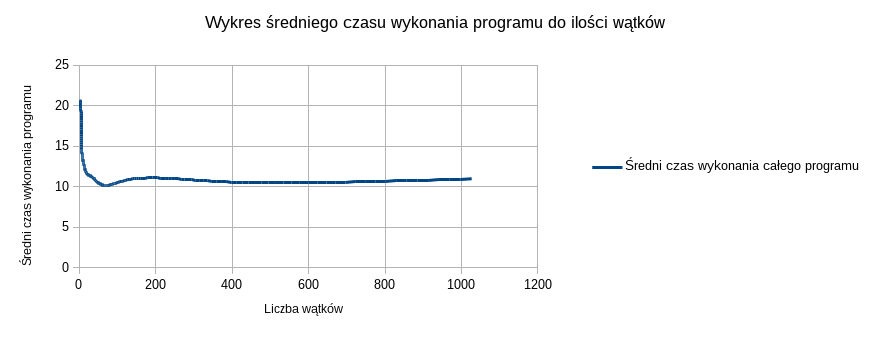
\includegraphics[width=0.7\textwidth]{data/wykonanieProgramu.png}
\end{center}

\begin{center}
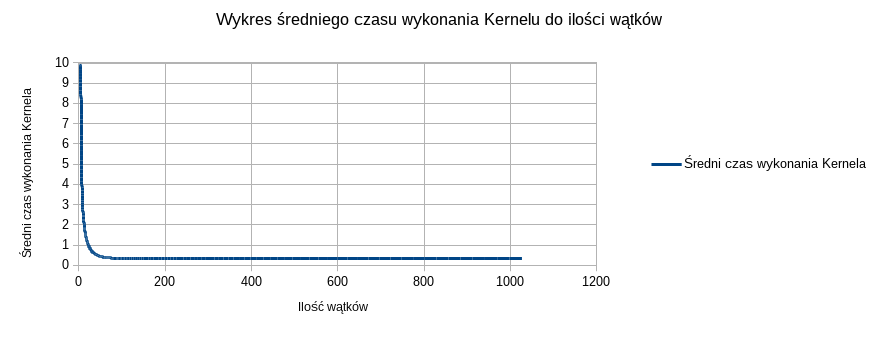
\includegraphics[width=0.7\textwidth]{data/wykonanieKernela.png}
\end{center}


\begin{center}
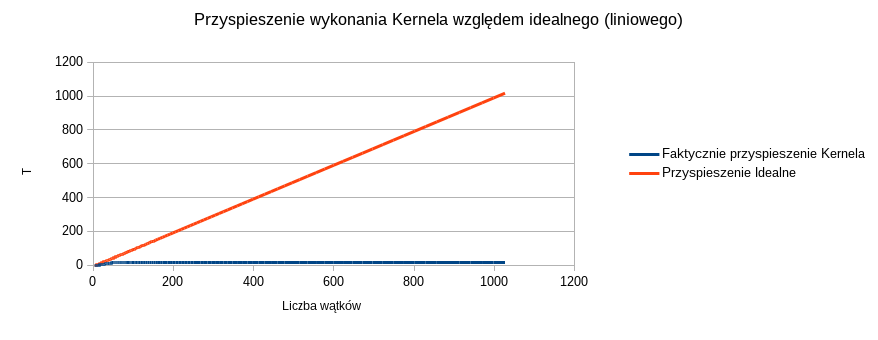
\includegraphics[width=0.7\textwidth]{data/przyspieszenie.png}
\end{center}

\section*{Wnioski}
Najlepsze przyspieszenie udało się osiągnąć dla 128 wątków (dla filmu Helicopter DivXHT ASP.divx). Jak widać nie da się osiągnąć większego przyspieszenia, bowiem rozmiar macierzy (klatki filmu) jest ograniczony i w pewnym momencie nie ma już możliwości dalszego dzielenia obliczen pomiedzy wątki. Dodatkowym obciążeniem mogą  być konieczności przełączania kontekstów, jednak nie udało nam się znaleźć jednoznacznego potwierdzenia istnienia takiego problemu dla procesorów GPU w literaturze przedmiotu.

\end{document}